% % % % % % % % % % % % % % % % % % % % % % % % % % % % % % % % % % % % %
% Chapter: Experiment 2
% % % % % % % % % % % % % % % % % % % % % % % % % % % % % % % % % % % % %
\chapter{Experiment 2: Smarter values generation}
\label{chp:experiment2}
% % % % % % % % % % % % % % % % % % % % % % % % % % % % % % % % % % % % %
% Section: Smarter values generation
%\section{Smarter values generation}
%\label{sec:ch4_smarter_values_generation}
\pinfo{Context - result of experiment 1, what aim is now}
Some bugs were found by using random input values in the first experiment. However the properties that use implication were not effectively checked in terms of the chance that the if-clause of the implicative properties were triggered when using random input values. This is what we aim to improve in this experiment, expecting to detect more bugs by triggering the implicative properties as expected.

% % % % % % % % % % % % % % % % % % % % % % % % % % % % % % % % % % % % %
% Section: Setup
\section{Setup}
\pinfo{2 categories separation}
We can separate the properties that we have in 2 different categories: those using implication ($\implies$) and those that do not. For each category we generate a test file, containing the tests belonging to that category. For the properties that use implication, another way of generating the random values would be more useful. We could optimize the random input values such that the if-clause of these properties are satisfied. When this is done, some these tests might end up failing too because the input values are now optimized for these cases. For the other category the earlier approach (random values as input) can still be used, we do not need to change this functionality for these cases.\\
\\
For the implication events the if-clause will be added to the preconditions, such that we can use those in order to generate the values matching this clause. When generating our test suit the events are being traversed, in case an event with some preconditions was found, it generates a test that is different than the earlier generated tests.\\
\\
The first difference is that it now uses our custom generator to determine the input values, instead of the build-in Java random generator. A list of tuples, containing values which satisfies the if-clause of the implication, are being generated. Our custom generator is a simple proof of concept in order to check if this will actually result in more failing tests. This custom generator basically consists of multiple methods which are being called based on the event name. In \autoref{lst:ch4_second_generating_values} this behavior is shown for the \textit{Symmetric} and \textit{Division1} event. The String parameter of these methods is a way how we can pattern match on the event name in Rascal. In case the event couldn't be handled, we throw an exception.
\\
\begin{sourcecode}[h!]
\begin{lstlisting}[language=Rascal]
private list[Expr] genTestValueForEvent("Symmetric") {
    Expr moneyValue = genRandomMoney();
    return [moneyValue, moneyValue];
}
private list[Expr] genTestValueForEvent("Division1") {
    real moneyAmountX = genRandomDouble();
    real intAmountY = genRandomInteger();
    real moneyAmountZ = moneyAmountX * intAmountY;
    str currency = genRandomCurrency();
    return [convertToMoney(currency, moneyAmountX), converToExpr(intAmountY), convertToMoney(currency, moneyAmountZ)];
}
private default list[Expr] genTestValueForEvent(str eventName) {
    throw "genTestValueForEvent not implemented for event <eventName>";
}
\end{lstlisting}
\caption{Values generation for \textit{Symmetric} and \textit{Division1}, including the fall-back case.}
\label{lst:ch4_second_generating_values}
\end{sourcecode}
\\
This means that the way how we determine these values is basically hard-coded, requiring to have knowledge about the if-clause itself. Note that this doesn't make this approach very dynamic, but the result will consist of a list of tuples that satisfy the if-clause. These tuples will be used as input for the test case that will be generated.\\
\\
However, these values are fixed when we translate them directly to a test, which completely removes the randomness of the values when running the tests. It would be nice to be able to run the tests such that the values are different on each run. To solve this problem, we can mutate the values in the list such that the values are sort of random again, while the tuples still satisfy the if-clause, as this was the actual intention. So the second difference is that for each tuple in the list, we will generate a random operation and use that to mutate the values inside the tuple. To ensure that the tuple values still satisfy the if-clause, each value will be mutated by the same operation. In \autoref{lst:ch4_second_resulting_test} an example of a generated test case is shown. The list of values are generated by using our custom generator, the amount of tuples in the list can be defined when generating the test suit. A method \code{genRandomOperation()} has been added to the template, which is used to mutate the fixed values in the list. After all the \code{checkAction()} method is being called to check the result of the test.
\\
\begin{sourcecode}[h!]
\begin{lstlisting}[language=Scala]
"work with Antisymmetry" in {
      Seq((USD(1593.62), USD(1593.62)), (USD(2869.78), USD(2869.78)),
          (EUR(4676.80), EUR(4676.80)), (USD(1850.29), USD(1850.29)),
          // ... // More values in the list
          (USD(9501.16), USD(9501.16)), (- EUR(149.67), - EUR(149.67)),
          (- EUR(159.67), - EUR(159.67)), (EUR(8015.77), EUR(8015.77)))
      .foreach {
        data:  (Money, Money) => {
          val randomOperation = genRandomOperation(genRandomOperator("Money", true), generateRandomMoney(data._1.currency), generateRandomInteger(true), generateRandomInteger(false), generateRandomPercentage(true), generateRandomPercentage(false), Random.nextInt(10))

          checkAction(Symmetry(
              randomOperation(data._1),
              randomOperation(data._2)
              )
          )
        }
      }
    }
\end{lstlisting}
\caption{Resulting test case with semi-random values. Omitted some input tuples for readability.}
\label{lst:ch4_second_resulting_test}
\end{sourcecode}
\\
Now that the input values for the implication events satisfy the if-clause, we can also update the specification such that the else-clause of the expression always returns \textit{False}. This results in a failing case again in case the precondition was not met. When this happens, it could indicate that there's a problem with our custom generator, or that the translation from the specification to the generated system was done incorrect.

% % % % % % % % % % % % % % % % % % % % % % % % % % % % % % % % % % % % %
% Section: Results
\section{Results}
\pinfo{Failing tests: Division}
Running the test suit with these changes resulted in an extra of 2 tests that were failing compared to the first experiment (\autoref{cpt:5_experiment1}). These were \textit{Division1} and \textit{Division2}, which reported that the precondition failed on the input values that were used, as shown in \autoref{lst:ch6_division_preconditionfailed}.
\\
\begin{sourcecode}[h!]
\begin{lstlisting}[language=Log]
[info] MoneyConditionsSpec
[info] - should work with Additive4params (7 seconds, 224 milliseconds)
[info] - should work with AntisymmetryLET (5 seconds, 493 milliseconds)
[info] - should work with Symmetric (5 seconds, 344 milliseconds)
[info] - should work with TransitiveInequalityLET (4 seconds, 343 milliseconds)
[info] - should work with AntisymmetryGET (5 seconds, 519 milliseconds)
[info] - should work with Additive (5 seconds, 26 milliseconds)
[info] - should work with TransitiveEquality (4 seconds, 423 milliseconds)
[info] - should work with TransitiveInequalityGET (4 seconds, 438 milliseconds)
[info] - should work with TransitiveInequalityLT (3 seconds, 792 milliseconds)
[info] - should work with TransitiveInequalityGT (3 seconds, 589 milliseconds)
[info] - should work with Division2 *** FAILED *** (23 milliseconds)
[info]   java.lang.AssertionError: assertion failed: expected CommandSuccess(Division2(-16729.90 USD,830,-20.16 USD)), found CommandFailed(NonEmptyList(PreConditionFailed(x == z*y)))
[info] - should work with Division1 *** FAILED *** (127 milliseconds)
[info]   java.lang.AssertionError: assertion failed: expected CommandSuccess(Division1(-44.68 USD,870,-38870.47 USD)), found CommandFailed(NonEmptyList(PreConditionFailed(x*y == z)))
[info]   ...
\end{lstlisting}
\caption{Precondition failed error in \textit{Division1} and \textit{Division2}.}
\label{lst:ch6_division_preconditionfailed}
\end{sourcecode}
\\
The values should be correct since we generated these values such that they match the if-clause of the implication properties. Note that the condition of the if-clause was added as preconditions in the specification, which causes these errors.\\
\\
\pinfo{Describe precision error happening at first}
For \textit{Division1} it states that the condition \code{x*y == z} failed. The values used for \textit{x}, \textit{y} and \textit{z} were \textit{-44.68 USD}, \textit{870} and \textit{-38870.47 USD} respectively. The result of \textit{x * y} = \textit{-44.68 USD * 870} = \textit{-38871.60 USD}. This should be equal to \textit{z}, in fact, the input of \textit{z} was slightly different, \textit{-38870.47 USD}. Remember that the input values are being mutated by a random operation that we have added to the test cases. This difference is caused by the precision error when operating with the \textit{Money} type, which we already found in \autoref{cpt:5_experiment1}. The random operation that was done was causing this behaviour. The same goes for the error with \textit{Division2}, where \code{x == z*y} should hold. The values of \textit{x}, \textit{y} and \textit{z} are \textit{-16729.90 USD}, \textit{830}, \textit{-20.16 USD} respectively. The result of \textit{z * y} = \textit{-16732.80 USD}, which is not equal to \textit{-16729.90} USD.\\
\\
\pinfo{Next (when fixed precision), division problem}
The first experiment already described the precision problem and how it could be fixed. We run these tests again against a new generated system (using the same generator) in which the precision errors that we identified earlier, are fixed. Running the test suit again on this system still results in the same amount of failing tests. As shown in Listing X, one case still fails on the precondition check, while the other case returns \textit{false}.

% % % % % % % % % % % % % % % % % % % % % % % % % % % % % % % % % % % % %
% Section: Analysis
\section{Analysis}
In this experiment we generated the input values such that the condition of the properties using implication are satisfied. When looking at the coverage report concerning a specific property, it can be seen that the else-clause of the implication is not being triggered any more. In \autoref{fig:ch6_eval_e2_highlighting_transitive-equality} the coverage of \textit{TransitiveEquality} is shown, note that only the else condition (which was translated to \textit{false}) is not triggered by the test suite. This was also the intention of the modification used in this experiment, as the if-clause is actually what we intended the property to check.
\\
\begin{figure}[h!]
\frame{
	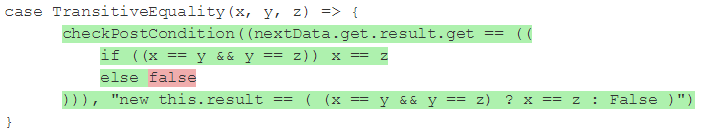
\includegraphics[width=\linewidth]{figures/eval_e2_transitive-equality}
}
\caption{Test coverage for \textit{TransitiveEquality} in second experiment}
\label{fig:ch6_eval_e2_highlighting_transitive-equality}
\centering
\end{figure}
\\
Although this did not lead to many additional bugs compared to the earlier experiment, there were still 2 additional failing tests related to the division problem. Both failing tests are related to the division problem that occurs when there is no even division of a number. For example: when dividing 1 by 3. When defining the specifications on the \textit{Money} type, we said that when this problem occurs, the value has to be rounded at the Xth \todo{Define x} decimal. However, these tests reveal that the generated system does not yet take this rule into account. Instead it tries to hold the exact value. As we have seen in Listing X \todo{Add listing}, one case (\textit{Division1}) fails because of a \code{PreconditionFailed} error, while \textit{Division2} passed the precondition check but results in \textit{false}. Since the \textit{Division2} test passes the precondition check in this example, it is probably the case that the calculated value tried to be used. The result check reveals that the property is still failing, meaning that it fails to hold the exact value. Which is understandable, as it has to be rounded somewhere, but it is not defined clearly yet. But this reveals that it is not the case that the rounding is done at the Xth \todo{Define x} decimal according to our definition.

% Evaluation criteria
\subsubsection{Evaluation criteria}
\pinfo{74\% on conditionals. Others remain the same - image}
The expectation was that the test suite could be improved, such that the test coverage on the SUT would become higher. In the first experiment we found that the properties using implication were not tested thoroughly. In this experiment these properties are triggering the if-clause of the properties using implication, thus we expect the test coverage to be higher when looking on the coverage of the properties. This is also follows from the results, as we can see in \autoref{fig:ch6_eval_experiment2}, the test coverage when looking at the logic file of the implicative properties is 74\%.
\\
\begin{figure}[h!]
\frame{
	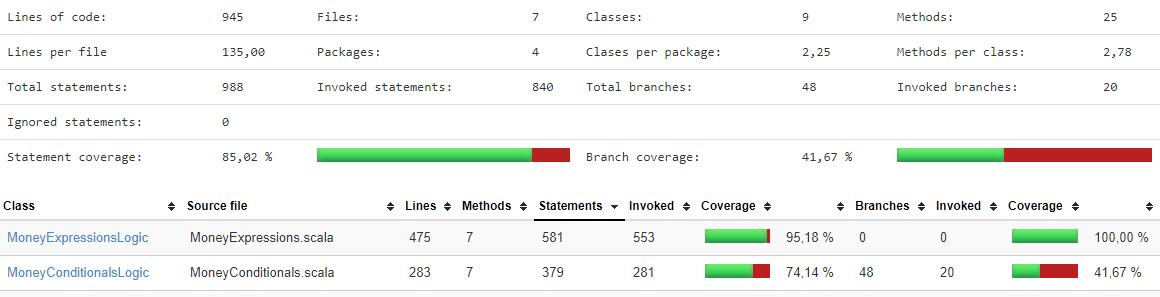
\includegraphics[width=\linewidth]{figures/eval_experiment2}
}
\caption{Test coverage report of the first experiment}
\label{fig:ch6_eval_experiment2}
\centering
\end{figure}
\\
\pinfo{Coverage, 85\% (overall), better}
The total test coverage on the SUT is reported to be 85\%. As we have discussed in the evaluation of the first experiment, we do not expect to reach the 100\% coverage, as there are certain components in the generated system which we do not test with this approach. Also, considering that the else-clause is not being triggered of the implicative properties, the test coverage will never become 100\%. Which is not a problem in that sense, as we don't intent to test the else clause, we are more interested in the result of the if-clause of these implicative properties.\\
\\
\pinfo{\# of bugs, 1 more}
The other criteria we use was the amount of bugs that we have found. Using this approach 2 more tests were failing compared to the first experiment in \autoref{cpt:5_experiment1}. The bug found was when using division with the \textit{Money} type, which is expected to be rounded off at the Xth decimal \todo{Define X}. However, as we have seen in this experiment, the generated system does not take this into account. We can categorize this bug into one category, rounding errors. These are different from precision errors as the precision errors are caused by having an incorrectly calculated value, where rounding errors are basically not working with the rounding method that is defined.

% % % % % % % % % % % % % % % % % % % % % % % % % % % % % % % % % % % % %
% Section: Threats to validity
\section{Threats to validity}
...
